\subsection*{4.1 Volume and Area}
\vspace{1em}
\noindent\markforreview
\vspace{1em}

Square A has side lengths that are \textbf{166} times the side lengths of square B.  
The area of square A is $k$ times the area of square B. What is the value of $k$?

\vspace{0.75em}

\vspace{2em}

\noindent\markforreview
\vspace{1em}

A cube has an edge length of 68 inches.  
A solid sphere with a radius of 34 inches is inside the cube, such that the sphere touches the center of each face of the cube.  
To the nearest cubic inch, what is the volume of the space in the cube \textit{not} taken up by the sphere?

\vspace{0.75em}

\choicebox{A}{149{,}796}  
\choicebox{B}{164{,}500}  
\choicebox{C}{190{,}955}  
\choicebox{D}{310{,}800}

\vspace{2em}
\newpage
\noindent\markforreview
\vspace{1em}

\begin{center}

\includegraphics[width=0.54\linewidth]{6.jpg}
\end{center}

The figure shown is a right circular cylinder with a radius of $r$ and height of $h$.  
A second right circular cylinder (not shown) has a volume that is 392 times as large as the volume of the cylinder shown.  
Which of the following could represent the radius $R$, in terms of $r$, and the height $H$, in terms of $h$, of the second cylinder?

\vspace{0.75em}

\choicebox{A}{$R = 8r$ and $H = 7h$}  
\choicebox{B}{$R = 8r$ and $H = 49h$}  
\choicebox{C}{$R = 7r$ and $H = 8h$}  
\choicebox{D}{$R = 49r$ and $H = 8h$}

\vspace{2em}

\noindent\markforreview
\vspace{1em}

A cube has a volume of 474{,}552 cubic units.  
What is the surface area, in square units, of the cube?

\vspace{0.75em}


\vspace{2em}

\noindent\markforreview
\vspace{1em}

A right circular cone has a height of 22 centimeters (cm) and a base with a diameter of 6 cm.  
The volume of this cone is $n\pi$ cm$^3$. What is the value of $n$?

\vspace{0.75em}



\vspace{2em}
\newpage
\noindent\markforreview
\vspace{1em}

A manufacturer determined that right cylindrical containers with a height that is 4 inches longer than the radius  
offer the optimal number of containers to be displayed on a shelf.  
Which of the following expresses the volume, $V$, in cubic inches, of such containers, where $r$ is the radius, in inches?

\vspace{0.75em}

\choicebox{A}{$V = 4\pi r^3$}  
\choicebox{B}{$V = \pi (2r)^3$}  
\choicebox{C}{$V = \pi r^2 + 4\pi r$}  
\choicebox{D}{$V = \pi r^3 + 4\pi r^2$}

\vspace{2em}

\noindent\markforreview
\vspace{1em}

A rectangular poster has an area of 360 square inches.  
A copy of the poster is made in which the length and width of the original poster are each increased by 20\%.  
What is the area of the copy, in square inches?

\vspace{0.75em}

\vspace{2em}

\noindent\markforreview
\vspace{1em}

A right rectangular prism has a length of \textbf{28 centimeters (cm)},  
a width of \textbf{15 cm}, and a height of \textbf{16 cm}.  
What is the surface area, in cm$^2$, of the right rectangular prism?

\vspace{0.75em}


\vspace{2em}
\newpage
\noindent\markforreview
\vspace{1em}

A right circular cone has a volume of $\dfrac{1}{3}\pi$ cubic feet and a height of \textbf{9 feet}.  
What is the radius, in feet, of the base of the cone?

\vspace{0.75em}

\choicebox{A}{$\dfrac{1}{3}$}  
\choicebox{B}{$\dfrac{1}{\sqrt{3}}$}  
\choicebox{C}{$\sqrt{3}$}  
\choicebox{D}{3}

\vspace{2em}


\noindent\markforreview
\vspace{1em}

Two identical rectangular prisms each have a height of $90$ centimeters (cm).  
The base of each prism is a square, and the surface area of each prism is $K\ \text{cm}^2$.  
If the prisms are glued together along a square base, the resulting prism has a surface area of $\frac{92}{47}K\ \text{cm}^2$.  
What is the side length, in cm, of each square base?

\vspace{0.75em}

\choicebox{A}{$4$}  
\choicebox{B}{$8$}  
\choicebox{C}{$9$}  
\choicebox{D}{$16$}

\vspace{2em}


\newpage
\noindent\markforreview
\vspace{1em}

The volume of right circular cylinder $A$ is $22$ cubic centimeters.  
What is the volume, in cubic centimeters, of a right circular cylinder with twice the radius and half the height of cylinder $A$?

\vspace{0.75em}

\choicebox{A}{$11$}  
\choicebox{B}{$22$}  
\choicebox{C}{$44$}  
\choicebox{D}{$66$}

\vspace{2em}
\noindent\markforreview
\begin{center}
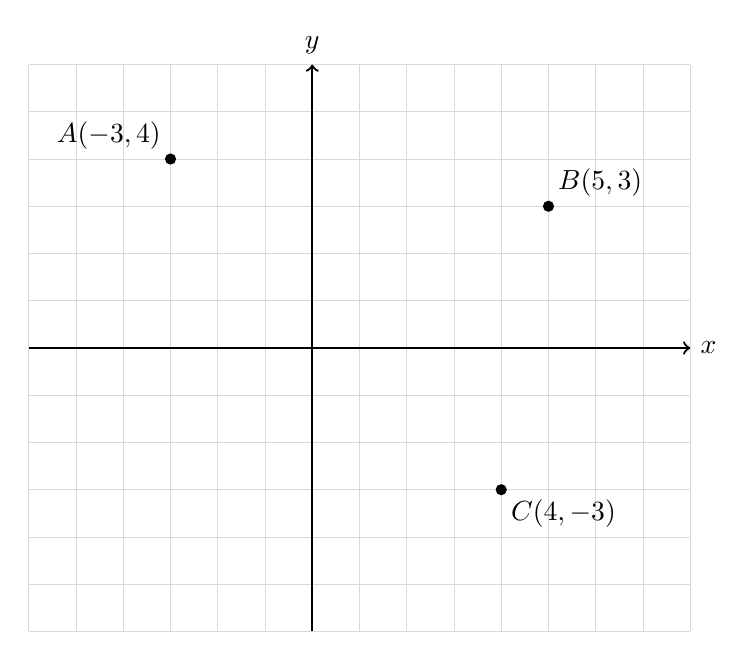
\begin{tikzpicture}[scale=0.6]
    % Draw grid
    \draw[very thin,color=gray!30] (-6,-6) grid (8,6);
    
    % Draw axes
    \draw[->,thick] (-6,0) -- (8,0) node[right] {$x$};
    \draw[->,thick] (0,-6) -- (0,6) node[above] {$y$};

    % Points
    \filldraw[black] (-3,4) circle (3pt) node[above left] {$A(-3,4)$};
    \filldraw[black] (5,3) circle (3pt) node[above right] {$B(5,3)$};
    \filldraw[black] (4,-3) circle (3pt) node[below right] {$C(4,-3)$};


\end{tikzpicture}
\end{center}




What is the area, in square units, of the triangle formed by connecting the three points shown?

\vspace{2em}

\newpage
\noindent\markforreview
\vspace{1em}

Circle $A$ has a radius of $3n$ and circle $B$ has a radius of $129n$, where $n$ is a positive constant.  
The area of circle $B$ is how many times the area of circle $A$?

\vspace{0.75em}

\choicebox{A}{$43$}  
\choicebox{B}{$86$}  
\choicebox{C}{$129$}  
\choicebox{D}{$1,849$}

\vspace{2em}

\noindent\markforreview
\vspace{1em}

The dimensions of a right rectangular prism are $4$ inches by $5$ inches by $6$ inches.  
What is the surface area, in square inches, of the prism?

\vspace{0.75em}

\choicebox{A}{$30$}  
\choicebox{B}{$74$}  
\choicebox{C}{$120$}  
\choicebox{D}{$148$}

\vspace{2em}

\newpage
\noindent\markforreview
\vspace{1em}

A right triangle has sides of length $2\sqrt{2}$, $6\sqrt{2}$, and $\sqrt{80}$ units.  
What is the area of the triangle, in square units?

\vspace{0.75em}



\choicebox{A}{$8\sqrt{2} + \sqrt{80}$}  
\choicebox{B}{$12$}  
\choicebox{C}{$24\sqrt{80}$}  
\choicebox{D}{$24$}

\vspace{2em}


\vspace{0.01mm}

\noindent\markforreview
\vspace{1em}

Triangles $ABC$ and $DEF$ are similar.  
Each side length of triangle $ABC$ is $4$ times the corresponding side length of triangle $DEF$.  
The area of triangle $ABC$ is $270$ square inches.  
What is the area, in square inches, of triangle $DEF$?

\vspace{2em}

\noindent\markforreview
\vspace{1em}

A cube has a surface area of $54$ square meters.  
What is the volume, in cubic meters, of the cube?

\vspace{0.75em}

\choicebox{A}{$18$}  
\choicebox{B}{$27$}  
\choicebox{C}{$36$}  
\choicebox{D}{$81$}

\newpage
